\section{Introduction}
Stencil codes are a class of algorithm in which array elements are updated based on the values within a fixed neighbourhood.
This pattern of computation occurs in a number of domains, including Computational Fluid Dynamics, Image processing and iterative linear solvers.

This paper presents the architectural pattern we refer to as Compute Array Streaming via Translation of Logical Elements (CASTLE).

\begin{figure}
  \booltrue{commstr}
  \booltrue{commstl}
  \booltrue{commsbr}
  \booltrue{commsbl}
  \centering
  \documentclass[tikz]{standalone}
\usepackage{etoolbox} % for toggles

\newbool{commstr}
\newbool{commstl}
\newbool{commsbr}
\newbool{commsbl}

\booltrue{commstr}
\booltrue{commstl}
\booltrue{commsbr}
\booltrue{commsbl}

\begin{document}
\tikzstyle{proc} = [circle, draw=black, fill=lightgray]

\begin{tikzpicture}[]
  \matrix[row sep=0.75cm, column sep=1.5cm] {
    \node (A3) [proc] {}; &  \node (B3) [proc] {}; &  \node (C3) [proc] {}; \\
    \node (A2) [proc] {}; &  \node (B2) [proc] {}; &  \node (C2) [proc] {}; \\
    \node (A1) [proc] {}; &  \node (B1) [proc] {}; &  \node (C1) [proc] {}; \\
  };
 
  % Vertical dashed continuity lines
  \path[->]
    (A1) edge[thick, dashed] (A2) 
    (B1) edge[thick, dashed] (B2)
    (C1) edge[thick, dashed] (C2)
    (A2) edge[thick, dashed] (A3) 
    (B2) edge[thick, dashed] (B3)
    (C2) edge[thick, dashed] (C3)
  ;
 
  % Bottom level --> arrows
  \ifbool{commsbr}{
    \path[->]
      (A1) edge[thick] (B2)
      (B1) edge[thick] (C2)
    ;
  }{}
  % Bottom level <-- arrows
  \ifbool{commsbl}{
    \path[->]
      (B1) edge[thick] (A2)
      (C1) edge[thick] (B2)
    ;
  }{}
  % Top level --> arrows
  \ifbool{commstr}{
    \path[->]
      (A2) edge[thick] (B3)
      (B2) edge[thick] (C3)
    ;
  }{}
  % Top level <-- arrows
  \ifbool{commstl}{
    \path[->]
      (B2) edge[thick] (A3)
      (C2) edge[thick] (B3)
    ;
  }{}
  \end{tikzpicture}
\end{document}

  \caption{Conventional Communications Pattern}
  \label{fig:convcomms}
\end{figure}

\begin{figure}
  \centering
  \documentclass[tikz]{standalone}

\begin{document}
  \tikzset{>=latex} % Change default arrowhead to filled triangle
  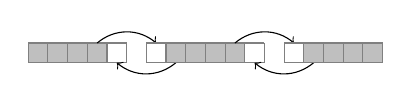
\begin{tikzpicture}[scale=0.25]
    \fill[lightgray] (0,0) rectangle (4,1);
    \draw[gray, step=1] (0,0) grid (5,1);
    
    \draw[->] (3.5,1) to [bend left=40] (6.5,1);
    \draw[->] (7.5,0) to [bend left=40] (4.5,0);

    \fill[lightgray] (7,0) rectangle (11,1);
    \draw[gray, step=1] (6,0) grid (12,1);
    
    \draw[->] (10.5,1) to [bend left=40] (13.5,1);
    \draw[->] (14.5,0) to [bend left=40] (11.5,0);

    \fill[lightgray] (14,0) rectangle (18,1);
    \draw[gray, step=1] (13,0) grid (18,1);

  \end{tikzpicture}
\end{document}

  \caption{Conventional 1D Boundary Exchange}
  \label{fig:exch1dold}
\end{figure}


\begin{figure}
  \centering
  \documentclass[tikz]{standalone}

\begin{document}
  \tikzset{>=latex} % Change default arrowhead to filled triangle
  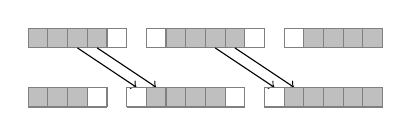
\begin{tikzpicture}[scale=0.25]

    % Timestep 1
    \fill[lightgray] (0,3) rectangle (4,4);
    \draw[gray, step=1] (0,3) grid (5,4);
    
    \fill[lightgray] (7,3) rectangle (11,4);
    \draw[gray, step=1] (6,3) grid (12,4);
    
    \fill[lightgray] (14,3) rectangle (18,4);
    \draw[gray, step=1] (13,3) grid (18,4);
   
   \draw[->](3.5,3) to (6.5,1);
   \draw[->](2.5,3) to (5.5,1);

   \draw[->](10.5,3) to (13.5,1);
   \draw[->](9.5,3) to (12.5,1);

    % Timestep 2
    \fill[lightgray] (0,0) rectangle (3,1);
    \draw[gray, step=1] (0,0) grid (4,1);
    
    \fill[lightgray] (6,0) rectangle (10,1);
    \draw[gray, step=1] (5,0) grid (11,1);
    
    \fill[lightgray] (13,0) rectangle (18,1);
    \draw[gray, step=1] (12,0) grid (18,1);


  \end{tikzpicture}
\end{document}

  \caption{Cascade 1D Boundary Exchange}
  \label{fig:trans1d}
\end{figure}


The contributions made in this research are:
\begin{itemize}
  \item{We introduce CASTLE and show how it can be applied to stencil codes;}
  \item{We show how CASTLE can be optimised for specific stencil codes and FPGA platforms.
        Specifically, we describe the various parameters which can be tuned to improve the performance of CASTLE.;}
  \item{We validate CASTLE by applying it to CODE-NAME-HERE, yielding a BIG-NUMERIC-IMPROVEMENT;}
\end{itemize}

Energy is also an important consideration for HPC applications and a key benefit of FPGA chips.
The fact that the hardware is not fixed opens up avenues of power optimisation.
Although both designs have the same runtime performance, the more frugal architecture places less demand on the power consumption.
<cite pose>

Important definition/term to include in the paper:
For an electronic circuit, a quiet state in which the circuit is driving no load and its inputs are not cycling. Most commonly used for the specification "quiescent current," the current consumed by a circuit when it in a quiescent state.

